\section{Simulation}

\subsection{Partie 1 -- Registre à décalage 4 bits}

\begin{figure}[H]
	\centering
	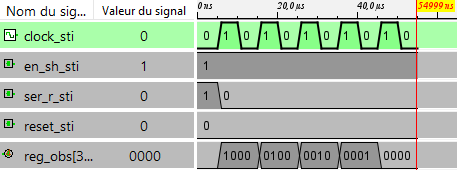
\includegraphics[width=\textwidth]{./images/simulation-partie1.png}
	\caption{Chronogramme de la simulation du registre à décalage 4 bits}
	\label{fig:simu_p1}
\end{figure}

Pour cette simulation, le reset est inactif et le décalage est activé en permanence (\texttt{en\_sh\_sti} = 1). Un 1 est appliqué sur l'entrée série \texttt{ser\_r\_sti} pendant la première période d'horloge, puis l'entrée repasse à 0. On observe sur \texttt{reg\_obs} que ce 1 entre par le bit de poids fort puis se décale d'une position vers la droite à chaque flanc montant de l'horloge : \texttt{1000}, \texttt{0100}, \texttt{0010}, \texttt{0001}, puis \texttt{0000} une fois sorti du registre. Le comportement correspond donc à celui attendu d'un registre à décalage à droite.

\subsection{Partie 2 -- Registre à décalage 8 bits}

% \begin{figure}[H]
% 	\centering
% 	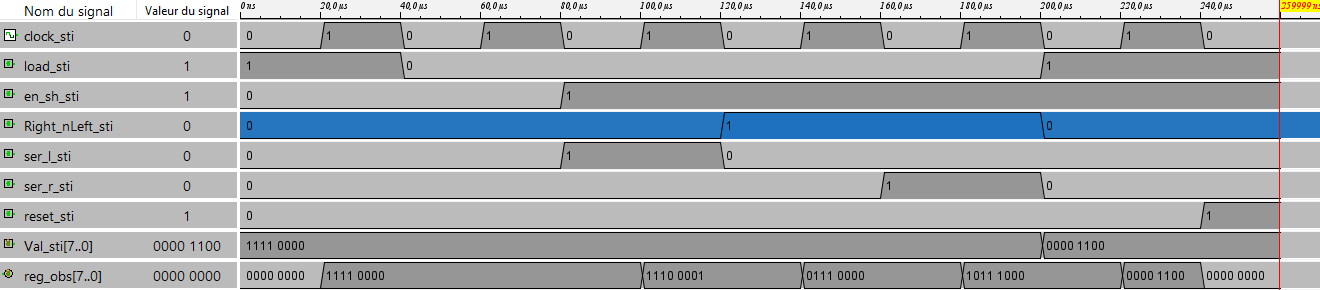
\includegraphics[width=\textwidth]{./images/simulation-partie2.png}
% 	\caption{Simulation du registre à décalage 8 bits}
% 	\label{fig:simu_p2}
% \end{figure}

\subsection{Partie 3 -- Chenillard}

% \begin{figure}[H]
% 	\centering
% 	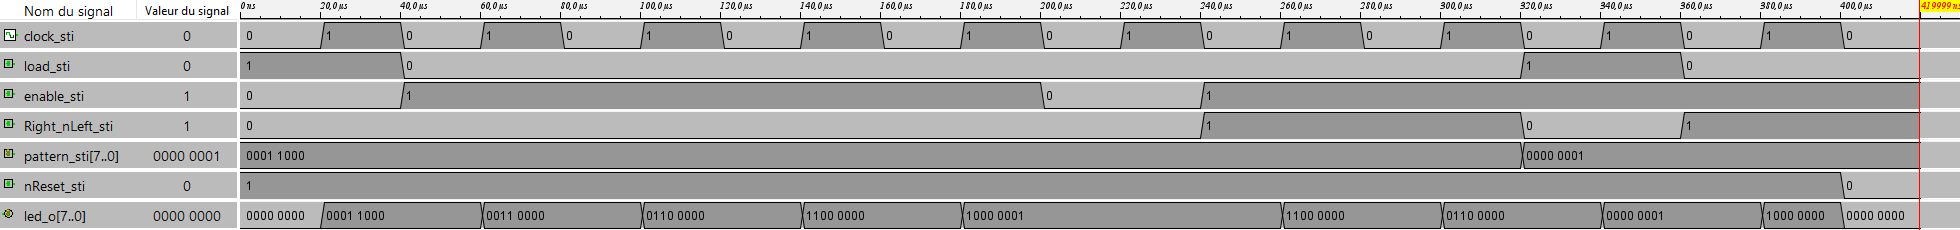
\includegraphics[width=\textwidth]{./images/simulation-partie3.png}
% 	\caption{Simulation du chenillard}
% 	\label{fig:simu_p3}
% \end{figure}
